\section{Background and Related Works}

\begin{figure}[t!]
    \centering
    \subfigure[Layered Architecture of Neural Network]
    {
        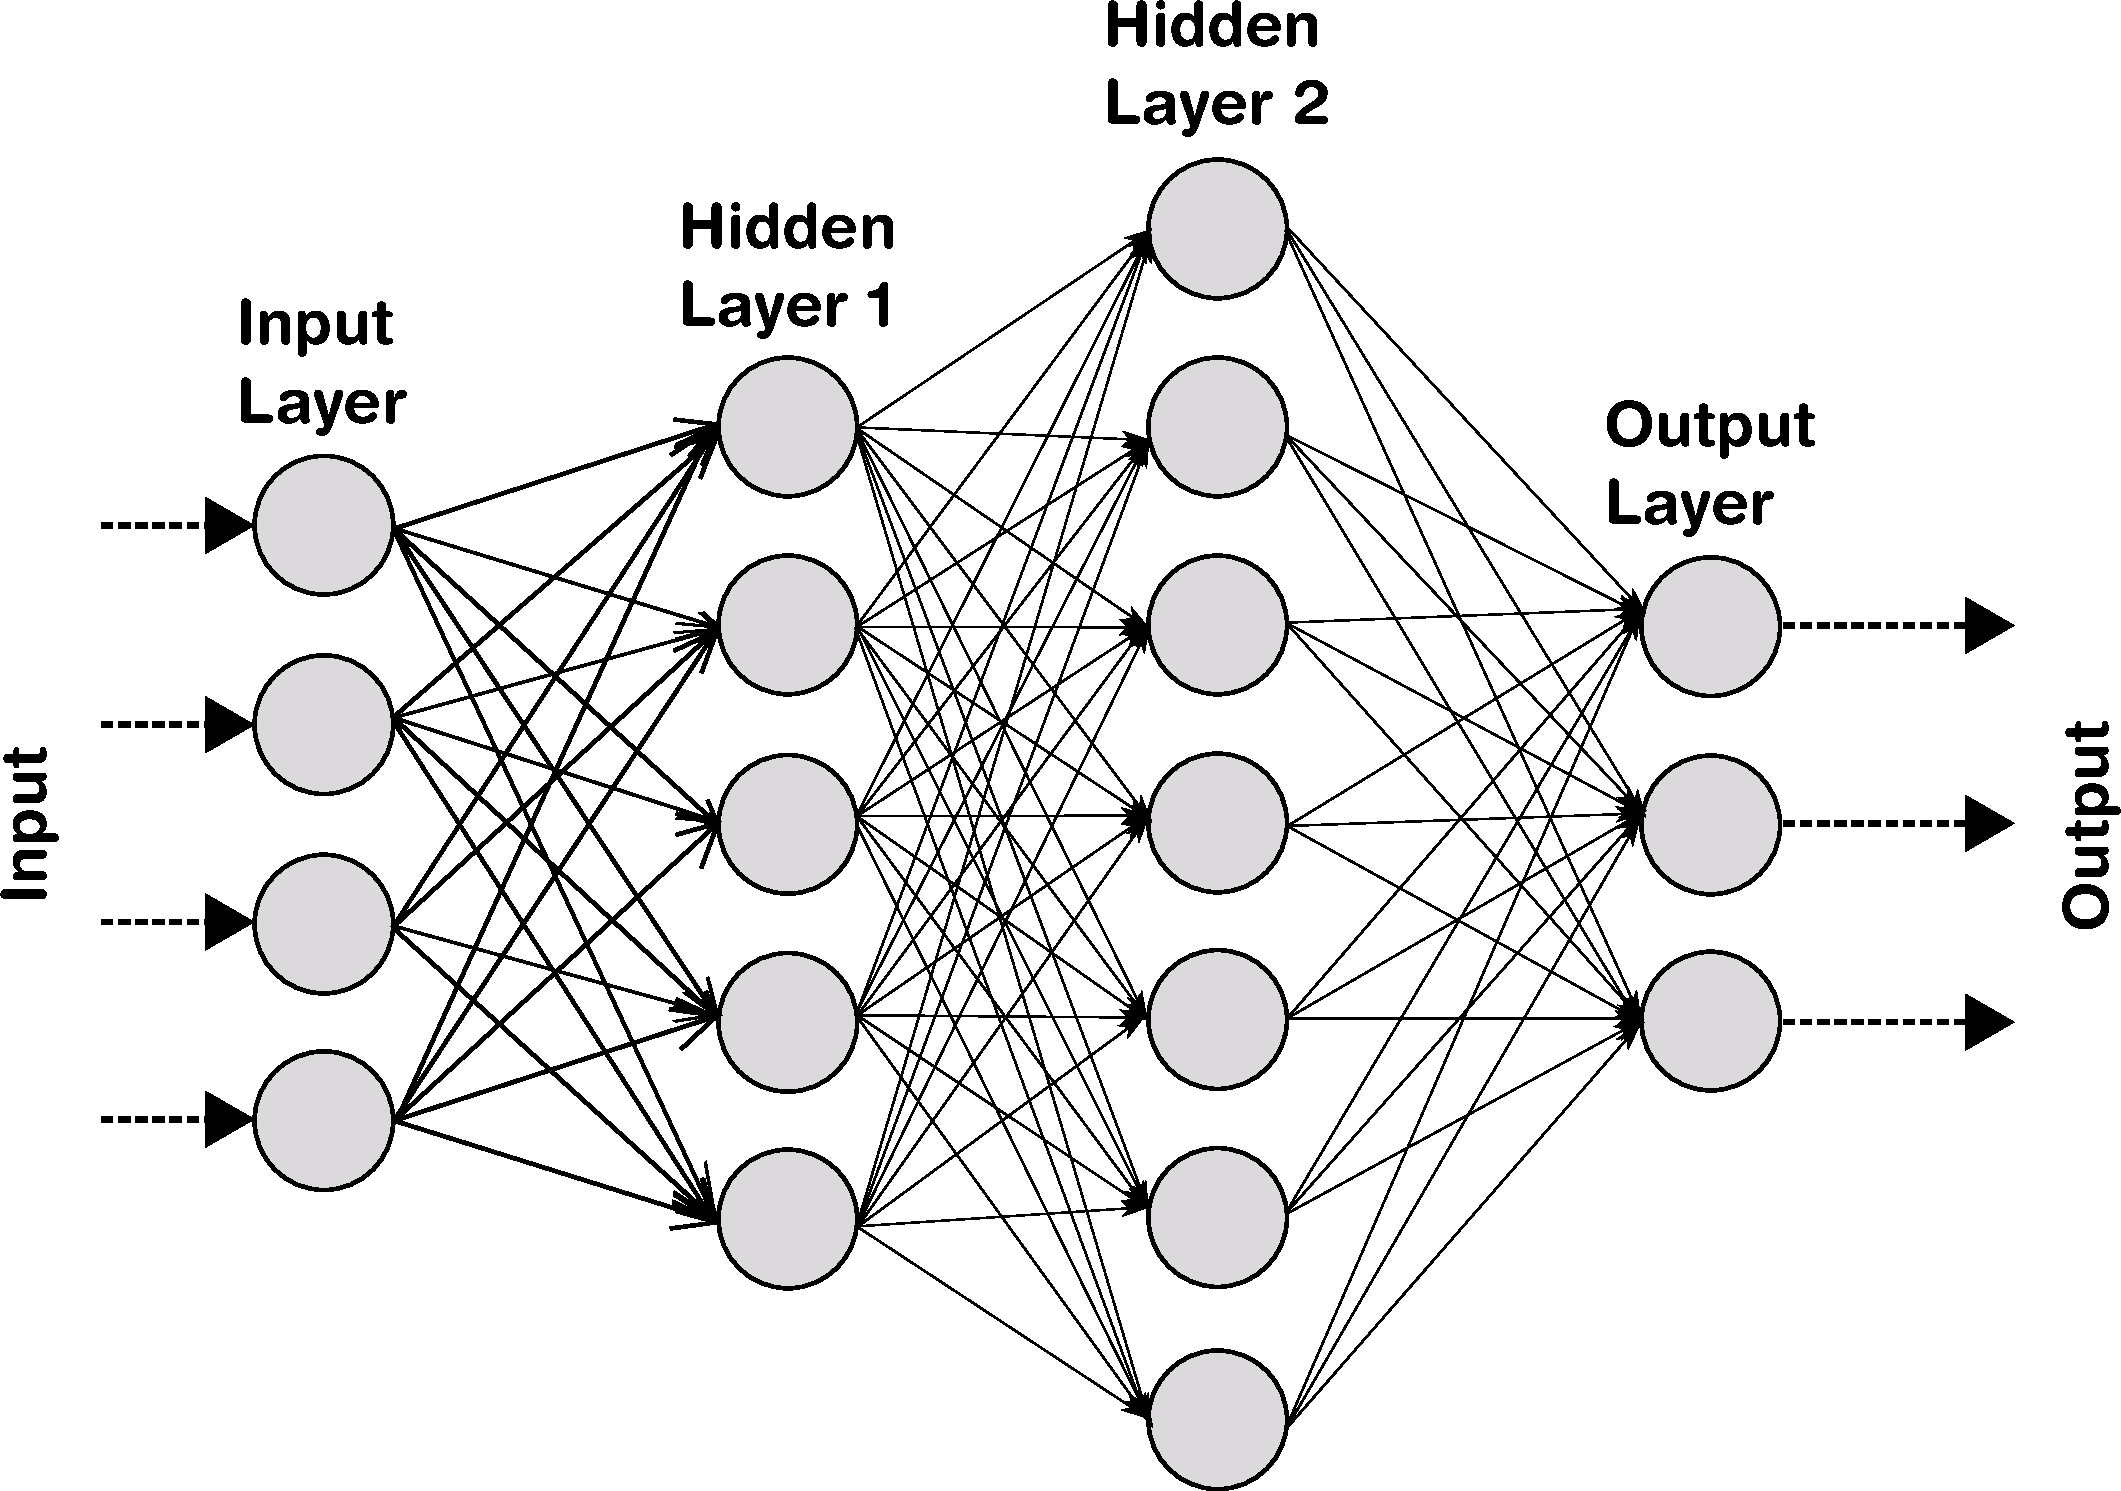
\includegraphics[width = 0.9\columnwidth]{Figures/NeuralNetwork.pdf}
        \label{fig:neuralNetwork}
    }
    \subfigure[A Single Artificial Neuron]
    {
        \label{fig:ann}
        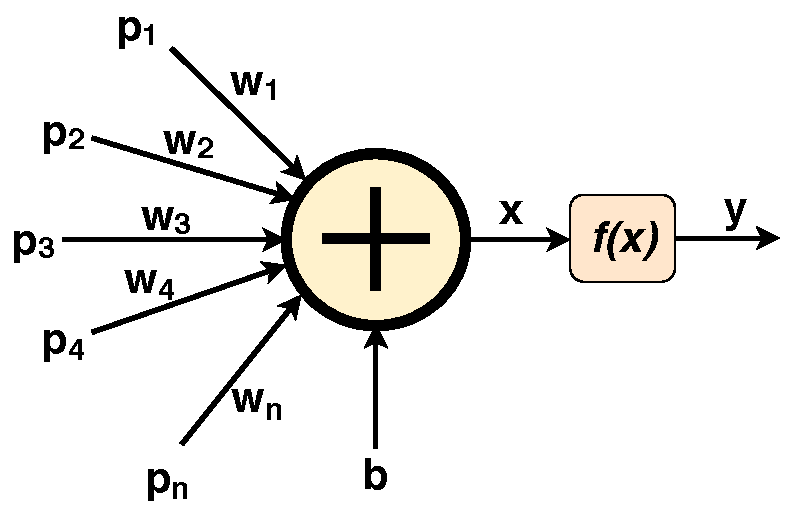
\includegraphics[width = 0.5\columnwidth]{Figures/ANN.pdf}
    }
    \caption{Architecture of a traditional feed-forward neural network and a single artifical neuron}
\end{figure}


~\cite{Furber2013}
Artificial Neural Networks~(ANNs) are inspired and adapted models of biological mammalian brain~\cite{}.
An ANN follows a layered architecture, where each layer is constructed form several neurons as shown in Fig.~\ref{fig:neuralNetwork}. 
In biological nervous system, signal transmission takes place between neurons through a structure called \emph{synapse} via electrical and chemical mechanisms. 
Synapse plays a vital role in determining the strength of connection between neurons.
Artificial neural networks emulate this behavior with the help of \emph{weights}.
Each connection~(synapse) between artificial neurons has a weight, which affects the signal passing though it by multiplying it with the weight. 
The weighted inputs are summed up in the neuron and passed to an activation function. 
Activation function transforms the input signals to output signals, and its main function is to make decision regarding how the output should behave to certain inputs. Fig.~\ref{fig:ann} depicts the neuron with the basic operations it performs. 

ANNs are consisted of many layers, which are classified into three groups: input layer, hidden layer and output layer. 
One layer can be fully or partially connected to the next layer. 
Hidden layer can be built from many intermediate layers between input an output.
Each input to the network is represented as a \emph{feature vector}.
For example in a handwriting recognition system using grayscale image, each input represents the brightness level of individual pixel in the picture.
Each neuron in the input layer represents one feature and there are no weights associated with input layer.

Traditional neural networks are \emph{feed forward} in nature where information moves in only in the forward direction.
More advanced architectures such as recurrent neural networks will have cyclic connections.
The networks are initially \emph{trained} to determine the values of different weights using training input samples.
Subsequently they are used with testing data for applications such as classification, pattern recognition and forecasting.

\subsection{Previous Works}

The hardware options utilized for machine learning are Central Processing Units (CPU), Graphic Processing Units (GPU), FPGA and Application-Specific Integrated Circuit (ASIC). Each of these options has their own advantages over others. CPUs are extremely flexible in terms of programmability, but they have issues regarding parallelism, cost and heat. GPUs have become most widely used hardware option for executing machine learning and deep learning tasks \cite{pooja2018}. They are designed to provide high level of parallelism, and thus well suits for the demand of machine and deep learning, where a lot of matrix multiplications and convolutions are involved. However, GPUs need to be incorporated with other chips (e.g. CPU, FPGA) that can rapidly execute NN on it (i.e. inference), since they are more suitable for training rather than inference. FPGAs have recently become popular for machine learning, and companies such as Microsoft and Baidu have invested in FPGAs heavily. FPGAs have much less power usage compared to CPUs, and their flexibility offers low latency and high bandwidth. Almost all implementations of ANN on FPGAs use various methods to utilize the reconfigurability of FPGA hardware. According to recent studies, FPGAs have outperformed GPUs in many applications, and it is predicated that they will soon be a better option than GPUs in deep learning \cite{pooja2018}. Even though ASICs are the least flexible among other above-mentioned hardware options, they compensate this drawback by offering highest efficiency. ASIC can be designed for both training or inference processes. 

There are many examples of ASIC that are designed to meet requirements of machine learning and ANN. Google’s Tensor Processing Unit (TPU) and IBM’s TrueNorth are the best examples of successful ASIC deployments for NN purposes. Being originally focused on 8-bit integers for inference tasks, TPUs now provides floating point precision and can be deployed in training as well \cite{pooja2018}. High performance and power efficiency of TPUs are achieved due to lack of extraneous logic \cite{pooja2018}. Hence, unlike other abovementioned hardware options, TPUs cannot be reprogrammed. IBM’s TrueNorth is a digital chip that consists of one million spiking-neurons incorporated with 256 million synapses. TrueNorth provides high efficiency due to spiking-neuron technology, and high scalability as several chips can be tiled in two-dimensions, as well as flexibility by offering independent configurability of individual neurons and synapses \cite{Merolla668}. TrueNorth is fabricated using CMOS technology and uses offline learning in NN purposes \cite{Merolla668}.
   

\subsection{Number Representation}

One critical factor in hardware implementation of ANN is the number representation of different data - synapse weights, biases and inputs/outputs of the neurons. Despite its widely usage in software ANNs, floating point arithmetic due to its prohibitively expensive cost is not well suited for hardware ANNs. As a result, the two's complement fixed binary point representation was chosen for data representation as it brings considerable optimization in terms of area usage and speed performance. However, this implies limited precision which is enough for many applications. Nevertheless, with this scheme learning process is accomplished off-chip in software using floating point representation. The conversions from decimal fractions to fixed point binary is done through equation~\ref{equation:dtob}.

\begin{equation}
b_{x}(d_{x})= \lfloor{d_{x}\cdot \frac{2^{n_{x}-1}-1}{2^{i_{x}-1}-2^{-f_{x}}}}\rceil
\label{equation:dtob}
\end{equation}
\begin{equation}
d_{x}(b_{x})= {b_{x}\cdot \frac{2^{i_{x}-1}-2^{-f_{x}}}{2^{n_{x}-1}-1}}
\label{equation:btod}
\end{equation}
Here, $n_{x}$, ${x}$, $f_{x}$ amount to total number of bits, integer bits and fractional bits of the given variable.